\documentclass[10pt]{article}

%% packages used
\usepackage{fullpage}
\usepackage{graphicx}
\usepackage{setspace}
\usepackage{hyperref}

%% packages not used
% \usepackage{ifthen}
% \usepackage{verbatim}
% \usepackage{pdfpages}




\title{Quantitative Methods for: Socialist Indoctrination in Venezuela}
\author{Ragan}

\begin{document}

\maketitle

\doublespace

\section{Literature}



\section{Methods}
The quantitative text analysis was preformed on the pre-Chavez and post-Chavez textbook sets. The textbooks were all in PDF format when we received them. The post-Chavez textbooks we already in machine readable form and we were able to directly read in those files for our text analysis. The pre-Chavez textbooks were also PDFs, but the text in these PDFs were not machine readable. We attempted to use various methods for converting the PDFs to a machine readable form using optical character recognition (OCR). The results from these attempts were always poor. In order to ensure that all the text from both textbooks sets was available for analysis we used the website Upwork.com to hire several Venezuelans to transcribe the PDFs to plain text for us. Once the pre-Chavez textbooks were transcribed we had five machine readable textbooks (Grade 1 - Grade 5) from both the pre-Chavez and post-Chavez eras. For both sets of textbooks the following steps were taken:\footnote{A detailed description of each step used in calculating the different metrics used in the quantitative analysis is included in the Appendix. Te R code used in the text analysis is available as an R Package that can be installed and run using the free R statistical language. The package can be found on GitHub at \url{https://github.com/robiRagan/prePostChavezTextbooks}}


\begin{enumerate}


\item Extract all words from the textbooks and store them along with the page number the word was located on. \label{beginSetDataFrameCreation}
	

\item Add the grade level to the data frame for each textbook and combine the five data frames into one data frame. \label{endSetDataFrameCreation}

\item Remove ``stop words", short words, underscores, whitespace, numeric digits, and words containing any stray characters. \label{stopWords}

\item Create Stems and Lemmas for all words so words with the same root are all categorized together as the same word. 


\item Calculate the proportions for all lemmas.

	\begin{enumerate}
	
	\item The overall proportions for each lemma are calculated using the following formula:
	
	$$ Prop.\ for\ Lemma_i = \frac{Frequency\ of\ Lemma_i}{\sum\limits_{i=1} Frequency\ of\ Lemma_i}$$
	
	\item The keyword proportions for each lemma are calculated using the following formula:
	
	$$ Prop.\ for\ Keyword\ Lemma_i = \frac{Frequency\ of\ Keyword\ Lemma_i}{\sum\limits_{i=1} Frequency\ of\ Keyword\ Lemma_i}$$
	
	\end{enumerate}
 

\item Calculate the change in proportion from pre-Chavez to post-Chavez for all lemmas.

	\begin{enumerate}
	
	\item The changes in the proportions are calculated using the following formula:
	
	$$ Change\ in\ Prop.\ for\ Lemma_i = Prop.\ for\ Lemma_i\ Post-Chavez - Prop.\ for\ Lemma_i\ Pre-Chavez $$
	
	\end{enumerate}


\item Calculate the change in proportion from pre-Chavez to post-Chavez for all key lemmas.

	\begin{enumerate}
	
	\item The changes in the proportions are calculated using the following formula:
	
	$$ Change\ in\ Prop.\ for\ Lemma_i = Prop.\ for\ Keyword\  Lemma_i\ Post-Chavez - Prop.\ for\ Keyword\ Lemma_i\ Pre-Chavez $$
	
	\end{enumerate}



\end{enumerate}






\section{Findings}

We analyze the lemma proportions in two ways. First we will look at all of the lemma proportions across the two textbook sets and then we will limit ourselves to a list of keywords. The list of keywords can be found in the appendix. 

\begin{figure}[h!]
  %\centering
  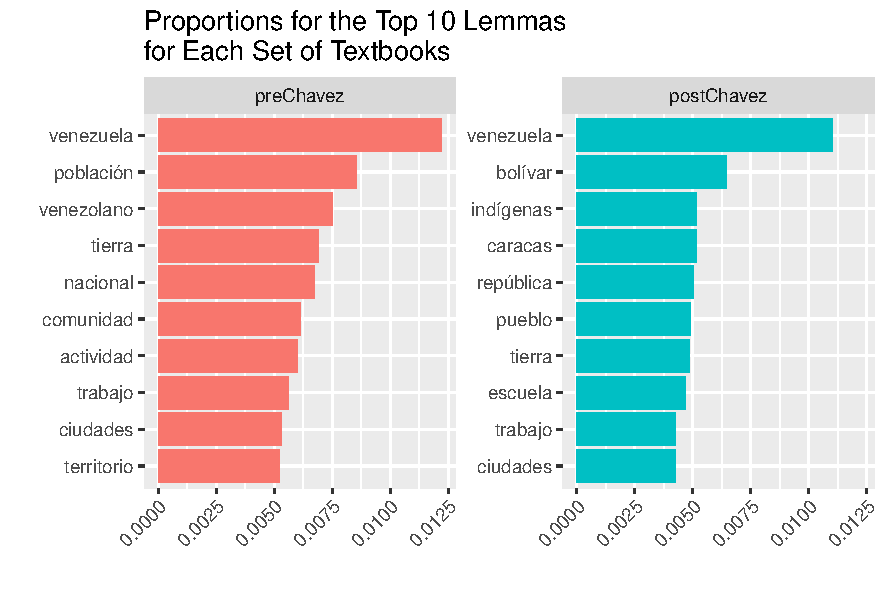
\includegraphics{images/top10AllLemmasProp}\\
  \caption{Top 10 Lemmas by Proportion\label{top10AllLemmasProp}}
\end{figure}

Figure \ref{top10AllLemmasProp} displays the ten highest lemma proportions for the two textbook sets. There is a great deal of difference between the most common lemmas used in the two sets. Only a few lemmas appear in both lists, ``venezuela",``ciudades", and``trabajo". The rest of the lemmas are unique. Of note is the frequent appearance of ``bol\'{i}var" in the Post-Chavez textbooks. The differences here could arise for any number of reasons and may not reflect the sort of ideological shift in elementary education we are interested in studying. To better gauge the shift in language form the Pre-Chavez to Post-Chavez era we limit the lemmas in our analysis to only a set of economic and social lemmas.\footnote{A full list of the keywords can be found in the appendix.} 


\begin{figure}[h!]
  %\centering
  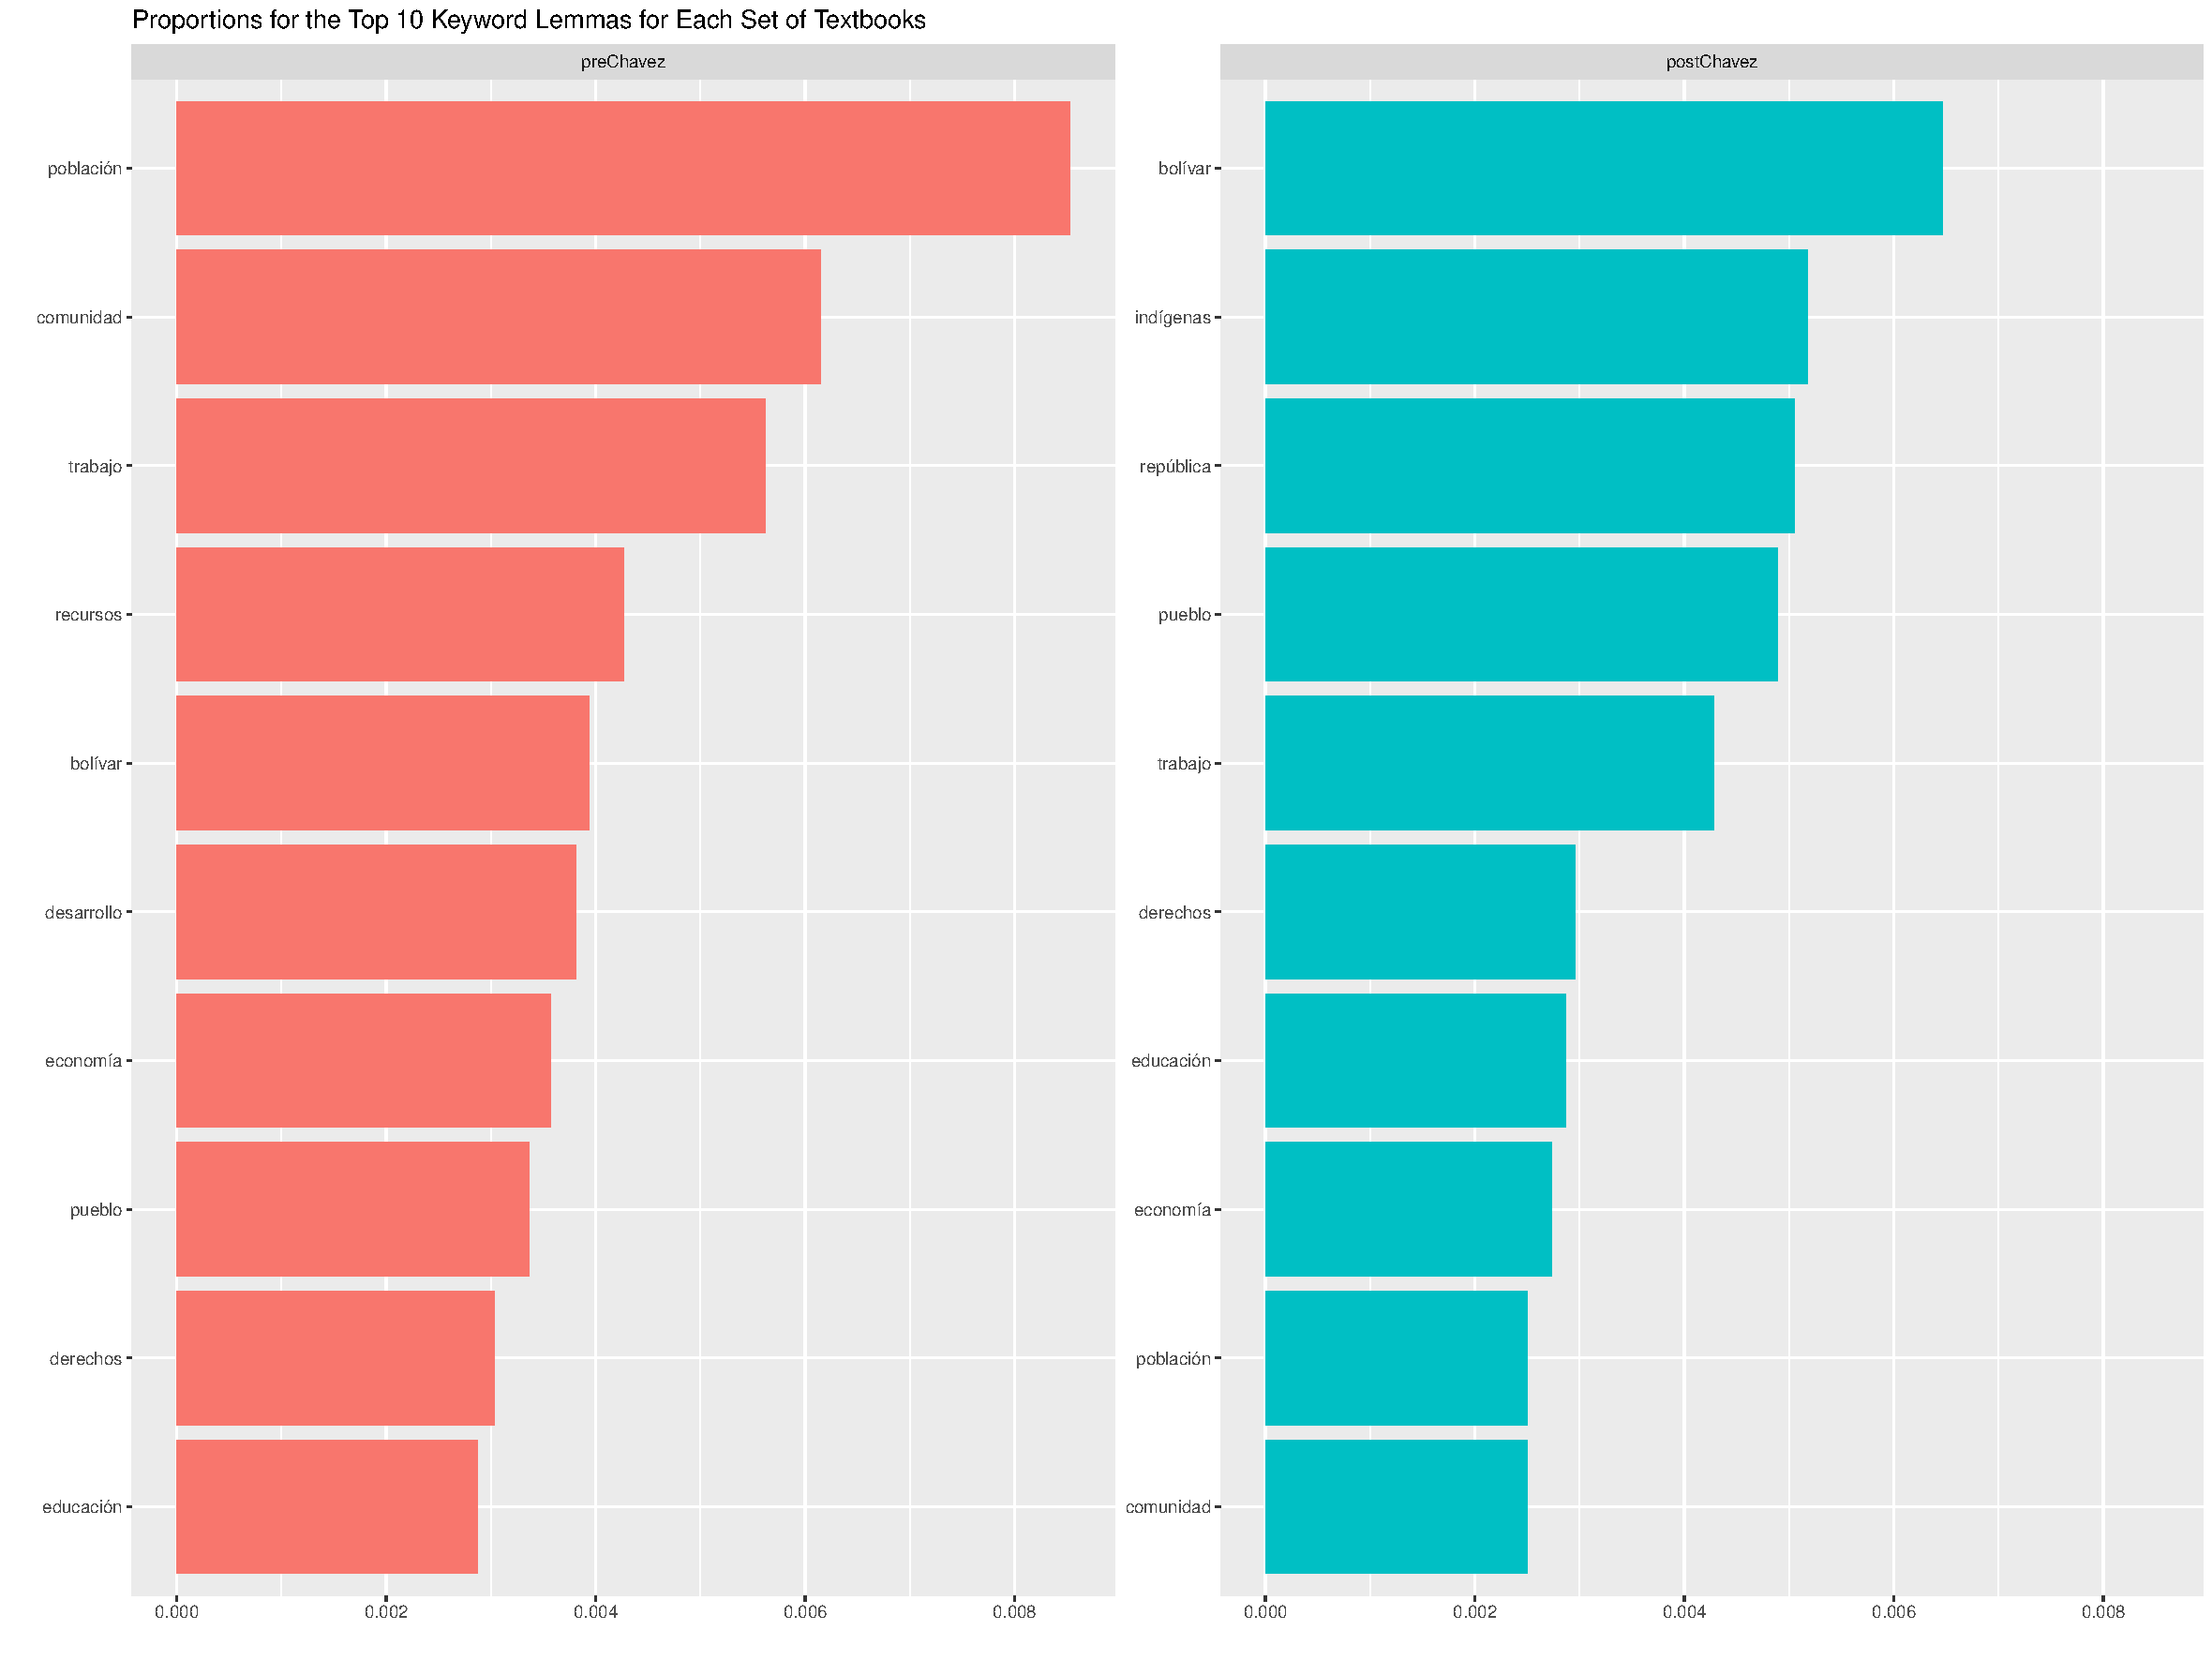
\includegraphics{images/top10KeywordLemmasProp}\\
  \caption{Top 10 Keyword Lemmas by Proportion\label{top10KeywordLemmasProp}}
\end{figure}

When we limit the lemmas to only those on our keyword list we now see more similarity across the two sets. But this is to be expected, because we have limited the set of lemmas to only those on our list. However, the differences across the two graphs now represent a much clearer picture of how language about economic and social issues in these textbooks has changed. For example ``poblac\'{i}on" was the lemma with the highest proportion in the Pre-Chavez textbook set, but it does not appear in the Top 10 of the Post-Chavez textbook set. On the other hand ``ind\'{i}genas" does not appear in the top 10 lemmas Pre-Chavez, but has the second highest keyword lemma proportion in the Post-Chavez textbooks. 

\clearpage

\begin{figure}[h!]
  %\centering
  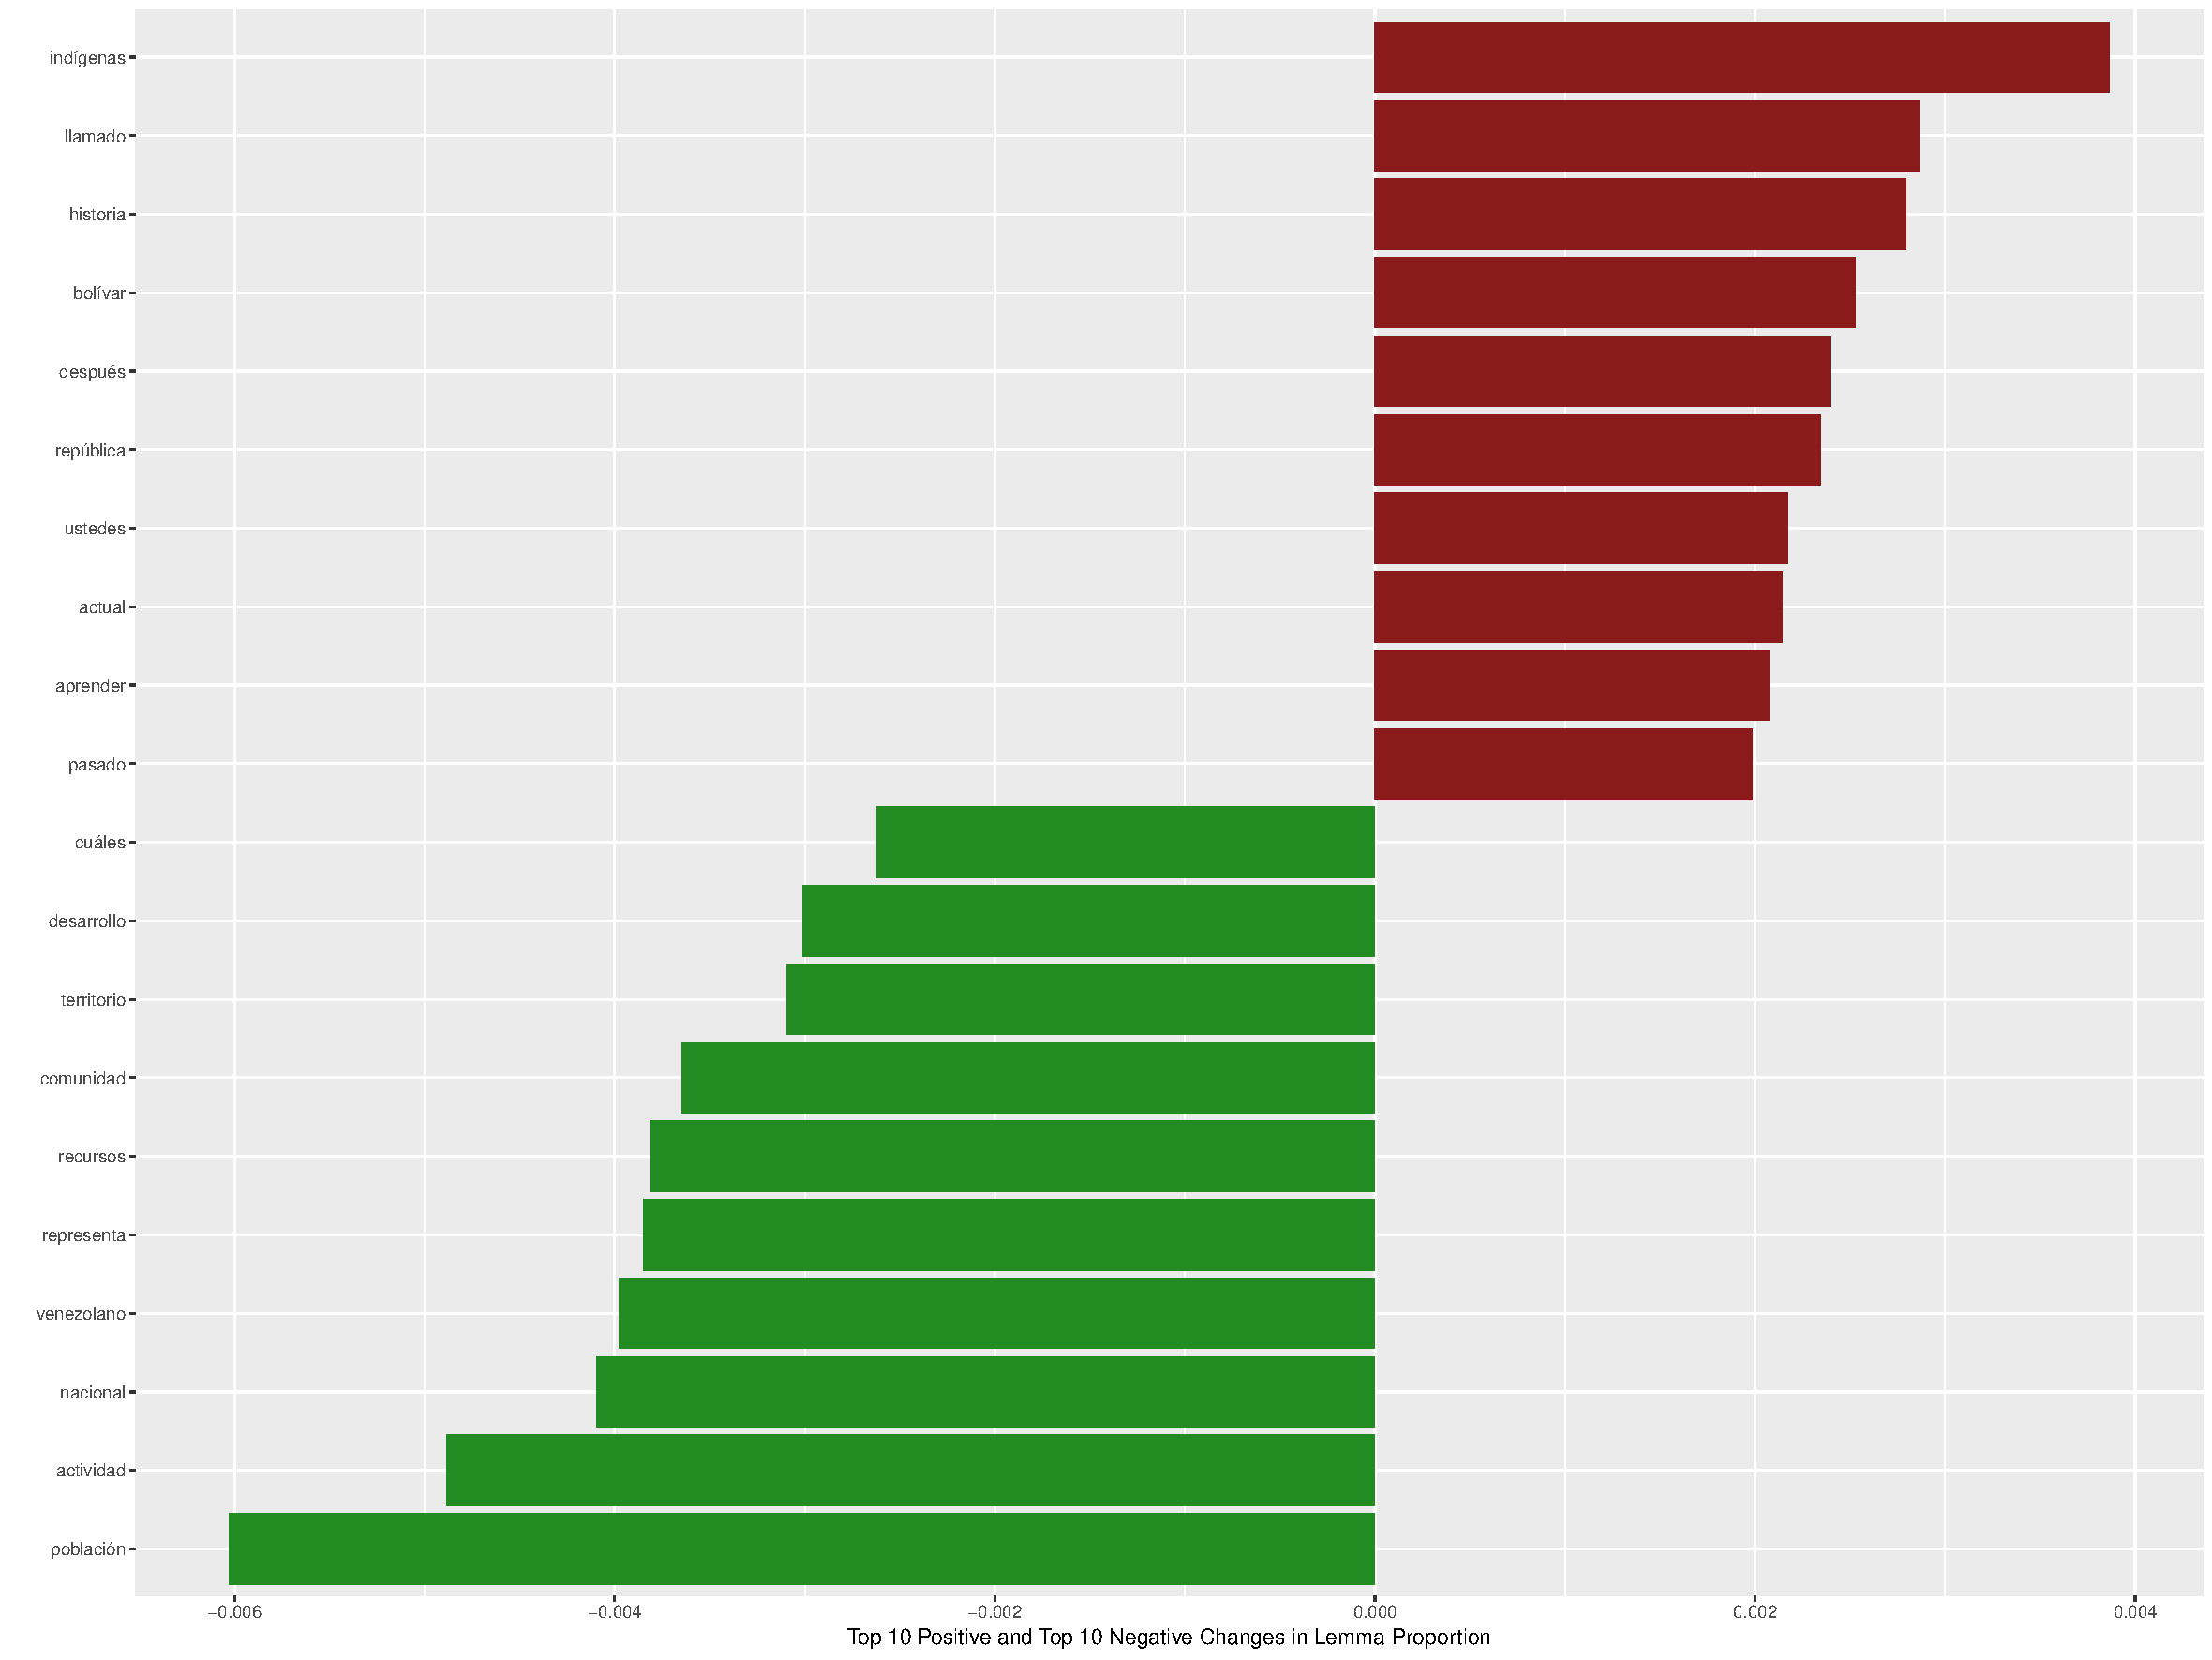
\includegraphics{images/top10AllLemmasPropChange}\\
  \caption{Change in All Lemmas Across the Two Textbook Sets\label{top10AllLemmasPropChange}}
\end{figure}

In Figure \ref{top10AllLemmasPropChange} we return to the set of all lemmas, not just the keyword lemmas. This graph looks at the lemmas whose proportion changed the most from the Pre-Chavez textbooks to the Post-Chavez Textbooks displays the ten highest lemma proportions for the two textbook sets. Here we see large increases in lemmas like, ``ind\'{i}genas",``bol\'{i}var", in line with the overall proportion graph. Lemmas like ``territorio", ``comunidad" and ``representa" see a large drop in their proportions. As before the changes in the proportions when looking at all lemmas may not hone in on changes in ideology as well as we would like them to. So we again limit the lemmas in our analysis to only a set of economic and social lemmas.


\clearpage

\begin{figure}[h!]
  %\centering
  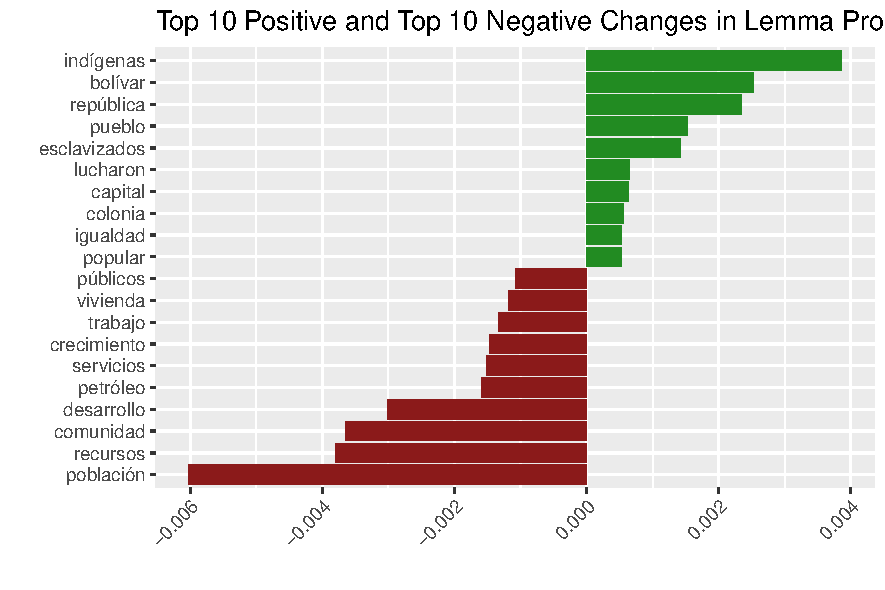
\includegraphics{images/top10KeywordsLemmasPropChange}\\
  \caption{Change in Keyword Lemmas Across the Two Textbook Sets \label{top10KeywordsLemmasPropChange}}
\end{figure}

In Figure \ref{top10KeywordsLemmasPropChange} we again limit the lemmas to only those on our keyword list we now see more similarity across the two sets. But this is to be expected, because we have limited the set of lemmas to only those on our list. The growth in the proportion for ``ind\'{i}genas" is still present here, as is the growth in the proportion for ``bol\'{i}var" and ``pueblo". In contrast terms like ``recursos", and ``vivienda" say their proportions fall. 
\newpage 

\section*{Appendix 1: Data Cleaning Details}
% \textbf{\textit{(Note: We may want to move some of the details from the data cleaning to an appendix. It is very detailed and long and may distract from the overall flow of the paper. But I think we do want to document it somewhere in the paper.)}}


% \textbf{\textit{(Note: We may want to move some of the details from the data cleaning to an appendix. It is very detailed and long and may distract from the overall flow of the paper. But I think we do want to document it somewhere in the paper.)}}
\begin{enumerate}


\item Extract all words from the textbook and store them along with the page number the word was located on. \label{beginSetDataFrameCreation}
	
	\begin{enumerate}
	\item The raw text from the PDF or Text file for a single textbook is read in and stored as an object. Here we will refer to this as \textbf{rawTextbookObject}. \label{beginTokenize}
	
	\item \textbf{rawTextbookObject} is then split with each page in the original text becoming its own data frame. Here we will refer to these as \textbf{rawPageDataFrames}.

	\item The \textbf{rawPageDataFrames} are stored as a single R list. With each page being a data frame that is one element of the R list. Here we will refer to this list as \textbf{rawPagesList}.

	\item For each page the raw text is tokenized. With each word receiving its own row in the first column of the data frame. The data frames will now be referred to as \textbf{tokenizedPageDataFrames} and the list storing all the data frames will be called \textbf{tokenizedPagesList}. 
	
	\item The second column in each of the \textbf{tokenizedPageDataFrames} contains the page number that each word appeared on. At this stage, each page has been converted to a two column data frame. The first column contains all the words on the page and the second column contains the page number the word appeared on. All of the \textbf{tokenizedPageDataFrames} are stored in an R list, \textbf{tokenizedPagesList}.

	\item All of the \textbf{tokenizedPageDataFrames} in \textbf{tokenizedPagesList} are merged into one data frame that contains all of the words in the textbook as the first column, and the page the word was found on as the second column. Here we will refer to this as \textbf{oneTokenizedTextbookDataFrame}.\label{endTokenize}
	
	\item Steps \ref{beginTokenize} through \ref{endTokenize} are run for each of the five textbooks in a set.
	\end{enumerate}

\item Add the grade level to the data frame for each textbook and combine the five data frames into one data frame. \label{endSetDataFrameCreation}

	\begin{enumerate}
	
	\item A third column is added to each \textbf{oneTokenizedTextbookDataFrame} that contains the grade level for the textbook. 
	
	\item The five \textbf{oneTokenizedTextbookDataFrame}s are all combined into one data frame. 
	
	\end{enumerate}


\item Steps \ref{beginSetDataFrameCreation} and \ref{endSetDataFrameCreation} above are run for the second set of five textbooks. The result is one data frame that contains all of the words from all five of the pre-Chavez textbooks, and one data frame that contains all of the words from all five of the post-Chavez textbooks.

\item Remove ``stop words", short words, underscores, whitespace, numeric digits, and words containing any stray characters. \label{stopWords}

	\begin{enumerate}
	
	\item Stop words are common short words that contain little information on their own. They are frequently discarded when doing text analysis on single words. The complete list of stop words is listed in an appendix. These words were all removed from the two data frames.
	
	\item Any word under five characters was removed form the analysis. Such words rarely provide any useful information on their own.
	
	\item Underscores and whitespace characters are sometimes generated when PDF files are read in for text analysis. These characters are removed.
	
	\item Numeric digits without any context contain little information, so such numbers are removed.
	
	\item When reading in text from a PDF file some words can contain stray characters like periods or numbers. This is usually due to an encoding issue with the way PDFs store some characters. Words with these stray characters are removed. In a related issue, the apostrophe symbol used in PDFs is encoded in a different way that the apostrophe symbol in text files. So all apostrophes were corrected to be the same across the two data frames.
	
	\end{enumerate}


\item Create Stems and Lemmas for all words.

	\begin{enumerate}
	
	\item Many words with the same meaning are not identical due to prefixes, suffixes or conjugation. For example in English the words``run" and ``running" would show up as different words in a word count, but in many cases we would want to count them in the same way. This is done through a process called Stemming and Lemmaing.
	
	\item Stemming basically takes words and reduces them to a shortened version of the word. For example the words: ``distribuci\'{o}n", ``distribuye", ``distribuida", ``distribuyen", ``distribuido", ``distribuidos", ``distribuirlas", and ``distribuyes" are all stemmed to become ``distribu".
	
	\item To create lemmas, we take the simple approach of assigning the most common word in a stem group as the lemma for all of the words in the stem group. For example, in the pre-Chavez data frame the stem family for ``boliv" contains the words ``bol\'{i}var" 327 times, ``bolivariana" 82 times, and bolivariano 1 time. So for this stem group the lemma is the most common word `bol\'{i}var". 
	
	\item All of the counts for the two textbook sets are based on the number of times a lemma appears in each textbook set. In the appendix we list some of the most common words across the data sets along with their stems and lemmas.
	
	\end{enumerate}


\item Calculate the proportions for all lemmas.

	\begin{enumerate}
	
	\item The proportions for each lemma are calculated using the following formula:
	
	$$ Prop.\ for\ Lemma_i = \frac{Frequency\ of\ Lemma_i}{\sum\limits_{i=1} Frequency\ of\ Lemma_i}$$
	
	\end{enumerate}


\item Calculate the change in proportion from pre-Chavez to post-Chavez for all lemmas.

	\begin{enumerate}
	
	\item The changes in the proportions are calculated using the following formula:
	
	$$ Change\ in\ Prop.\ for\ Lemma_i = Prop.\ for\ Lemma_i\ Post-Chavez - Prop.\ for\ Lemma_i\ Pre-Chavez $$
	
	\end{enumerate}



\end{enumerate}

\section*{Appendix 2: Stop Words}
\textbf{\textit{(NOTE: Accent marks and other non-english characters are giving LaTeX problems make sure to double check this list)}}

The stop words used in Step \ref{stopWords} of the data cleaning:

de, la, que, el, en, y, a, los, del, se, las, por, un, para, con, no, una, su, al, lo, como, m�s, pero, sus, le, ya, o, este, s\'{i}, porque, esta, entre, cuando, muy, sin, sobre, tambi\'{e}n, me, hasta, hay, donde, quien, desde, todo, nos, durante, todos, uno, les, ni, contra, otros, ese, eso, ante, ellos, e, esto, m\'{i}, antes, algunos, qu\'{e}, unos, yo, otro, otras, otra, \'{e}l, tanto, esa, estos, mucho, quienes, nada, muchos, cual, poco, ella, estar, estas, algunas, algo, nosotros, mi, mis, t\'{u}, te, ti, tu, tus, ellas, nosotras, vosotros, vosotras, os, m\'{i}o, m\'{i}a, m\'{i}os, m\'{i}as, tuyo, tuya, tuyos, tuyas, suyo, suya, suyos, suyas, nuestro, nuestra, nuestros, nuestras, vuestro, vuestra, vuestros, vuestras, esos, esas, estoy, est�s, est�, estamos, est�is, est�n, est\'{e}, est\'{e}s, estemos, est\'{e}is, est\'{e}n, estar\'{e}, estar�s, estar�, estaremos, estar\'{e}is, estar�n, estar\'{i}a, estar\'{i}as, estar\'{i}amos, estar\'{i}ais, estar\'{i}an, estaba, estabas, est�bamos, estabais, estaban, estuve, estuviste, estuvo, estuvimos, estuvisteis, estuvieron, estuviera, estuvieras, estuvi\'{e}ramos ,estuvierais, estuvieran, estuviese, estuvieses, estuvi\'{e}semos, estuvieseis, estuviesen, estando, estado, estada, estados, estadas, estad, he, has, ha, hemos, hab\'{e}is, han, haya, hayas, hayamos, hay�is, hayan, habr\'{e}, habr�s, habr�, habremos, habr\'{e}is, habr�n, habr\'{i}a, habr\'{i}as, habr\'{i}amos, habr\'{i}ais, habr\'{i}an, hab\'{i}a, hab\'{i}as, hab\'{i}amos, hab\'{i}ais, hab\'{i}an, hube, hubiste, hubo, hubimos, hubisteis, hubieron, hubiera, hubieras, hubi\'{e}ramos, hubierais, hubieran, hubiese, hubieses, hubi\'{e}semos, hubieseis, hubiesen, habiendo, habido, habida, habidos, habidas, soy, eres, es, somos, sois, son, sea, seas, seamos, se�is, sean, ser\'{e}, ser�s, ser�, seremos, ser\'{e}is, ser�n, ser\'{i}a, ser\'{i}as, ser\'{i}amos, ser\'{i}ais, ser\'{i}an, era, eras, \'{e}ramos, erais, eran, fui, fuiste, fue, fuimos, fuisteis, fueron, fuera, fueras, fu\'{e}ramos, fuerais, fueran, fuese, fueses, fu\'{e}semos, fueseis, fuesen, siendo, sido, tengo, tienes, tiene, tenemos, ten\'{e}is, tienen, tenga, tengas, tengamos, teng�is, tengan, tendr\'{e}, tendr�s, tendr�, tendremos, tendr\'{e}is, tendr�n, tendr\'{i}a, tendr\'{i}as, tendr\'{i}amos, tendr\'{i}ais, tendr\'{i}an, ten\'{i}a, ten\'{i}as, ten\'{i}amos, ten\'{i}ais, ten\'{i}an, tuve, tuviste, tuvo, tuvimos, tuvisteis, tuvieron, tuviera, tuvieras, tuvi\'{e}ramos, tuvierais, tuvieran, tuviese, tuvieses, tuvi\'{e}semos, tuvieseis, tuviesen, teniendo, tenido, tenida, tenidos, tenidas, tened.


\section*{Appendix 3: Examples of Stems and Lemmas}
\textbf{\textit{(NOTE: Accent marks and other non-english characters are giving LaTeX problems make sure to double check this list)}}
\begin{table}[h]
\centering
\begin{tabular}{l|c|c}
 \textbf{word}			& \textbf{stem}		& \textbf{lemma}		\\
 \hline                                     
 venezuela     			& venezuel    		& venezuela    		\\
 bol\'{i}var       		& boliv       		& bol\'{i}var      	\\
 caracas       			& carac       		& caracas      		\\
 escuela       			& escuel      		& escuela      		\\
 despu\'{e}s       		& despues     		& despu\'{e}s		\\
 rep\'{u}blica     		& republ      		& rep\'{u}blica    	\\
 historia      			& histori     		& historia     		\\
 tiempo        			& tiemp       		& tiempo       		\\
 ind\'{i}genas     		& indigen     		& ind\'{i}genas    	\\
 tierra        			& tierr       		& tierra       		\\
 pueblo        			& puebl       		& pueblo       		\\
 am\'{e}rica       		& amer        		& am\'{e}rica      	\\
 espa\~{n}a        		& espa\~{n}       	& espa\~{n}a       	\\
 personas      			& person      		& personas     		\\
 poblaci\'{o}n     		& poblacion   		& poblaci\'{o}n    	\\
 ciudad        			& ciud        		& ciudades     		\\
 nacional      			& nacional    		& nacional     		\\
 comunidad     			& comun       		& comunidad    		\\
 familia       			& famili      		& familia      		\\
 ustedes       			& usted       		& ustedes      		\\
 trabajo       			& trabaj      		& trabajo      		\\
 educaci\'{o}n     		& educ        		& educaci\'{o}n    	\\
 ind\'{i}gena      		& indigen     		& ind\'{i}genas    	\\
 independencia 			& independent 		& independencia		\\
 territorio    			& territori   		& territorio   		\\
\end{tabular}
\end{table}



\section*{Appendix 4: Keywords}
\textbf{\textit{(NOTE: Accent marks and other non-english characters are giving LaTeX problems make sure to double check this list)}}
\begin{small}

\begin{table}[h]
\centering
\begin{tabular}{l|c| |l|c}
Category  							&     	Keyword           &   Category          &      Keyword                          \\
\hline                                                                                             
surplus value  						&     	abuso             &   public goods  	&     	bienes           \\
surplus value  						&     	apropiaci\'{o}n   &   public goods  	&     	p\'{u}blicos     \\
surplus value  						&     	aprovechar        &   public goods  	&     	bienestar        \\
surplus value  						&     	capital           &   public goods  	&     	educaci\'{o}n    \\
surplus value  						&     	despojo           &   public goods  	&     	explotaci\'{o}n  \\
surplus value  						&     	obreros           &   public goods  	&     	gratis           \\
objective theory of value  			&     	costo             &   public goods  	&     	gratuita         \\
objective theory of value  			&     	injusto           &   public goods  	&     	salud            \\
objective theory of value  			&     	justo             &   public goods  	&     	servicios        \\
objective theory of value  			&     	trabajo           &   public goods  	&     	vivienda         \\
objective theory of value  			&     	esclavo           &   nationalism  		&     	bol\'{i}var      \\
subjective theory of value  		&     	oferta            &   nationalism  		&     	patria           \\
subjective theory of value  		&     	demanda           &   nationalism  		&     	Latinoam�rica    \\
subjective theory of value  		&     	precio            &   nationalism  		&     	rep\'{u}blica    \\
subjective theory of value  		&     	mercado           &   nationalism  		&     	Venezuela        \\
income/wealth redistribution  		&     	comunidad         &   nationalism  		&     	colonia          \\
income/wealth redistribution  		&     	derecho           &   production  		&     	crecimiento      \\
income/wealth redistribution  		&     	desigualdad       &   production  		&     	desarrollo       \\
income/wealth redistribution  		&     	distribuci\'{o}n  &   production  		&     	recursos         \\
income/wealth redistribution  		&     	igualdad          &   production  		&     	poblaci\'{o}n    \\
income/wealth redistribution  		&     	injusticia        &   production  		&     	econom\'{i}a     \\
income/wealth redistribution  		&     	justicia          &   production  		&     	petr\'{o}leo     \\
income/wealth redistribution  		&     	repartici\'{o}n   &                   	&                        \\
income/wealth redistribution  		&     	ind\'{i}gena      &                   	&                        \\
income/wealth redistribution  		&     	pueblo            &                   	&                        \\
income/wealth redistribution  		&     	lucha             &                   	&                        \\
income/wealth redistribution  		&     	popular           &                   	&                           
\end{tabular}
\end{table}

\end{small}



%\newpage
%\bibliography{bib.bib}
%\bibliographystyle{apsr}


\end{document}


# Generic Code to Insert Figures:

%\begin{figure}[h!]
%  \centering
%  \includegraphics[width=4in]{"filename"}\\
%  \caption{caption}
%\end{figure}